\documentclass[supercite]{HustGraduPaper}
%进行个人信息设置
\title{阿尔茨海默症患者肠道菌群16S 测序数据分析} %论文题目
\author{苏济雄} %作者姓名
\date{\today} %日期,默认当日
\school{生命科学与技术学院} %院系名称
\classnum{生信基地1801班} %专业班级
\stunum {U201812416} %学号
\instructor{宁康} %指导教师姓名

%添加自己要用的其他宏包
\usepackage{xltxtra}
\usepackage{bm}
\usepackage{caption}
\captionsetup{font={scriptsize}}
\usepackage{graphicx}
\usepackage{float}
\begin{document}
%生成标题页 \maketitle[可选参数]
%可选参数:
%logo color=green/black 华中科技大学字样的颜色,绿色或者黑色,默认绿色
%line length=12em 填写信息处横线的长度,默认12em
%line font=huawenzhongsong 填写信息的字体,默认huawenzhongsong
\maketitle

%生成声明与授权书页 \statement[可选参数]
%可选参数:
%confidentiality=yes/no/true/false/empty 是否保密,yes/true为保密;no/false为不保密,empty为不填,默认为empty
%year=5 保密年数,默认为空
% \statement

\clearpage %结束上一页
\pagenumbering{Roman} %摘要页码为大写罗马数字

%填写中文摘要内容和关键字
% \begin{cnabstract}{阿尔茨海默症;16S 扩增子测序;差异分析}
% 	目前已有许多研究发现肠道菌群通过肠-脑轴影响中枢神经系统,在 AD 患者认知功能、精神行为症状的发生发展中有重要的作用;另外,肠道菌群与 AD 临床标志物存在密切关联,通过改善 AD 患者肠道菌群也可以改善认知功能。本文尝试通过对公共数据库收集的 AD 患者肠道菌群 16S 扩增子测序数据进行分析,探索其与健康对照组的组成和功能差异。
% \end{cnabstract}
%填写英文摘要内容和关键字
% \begin{enabstract}{Key1; Key2; Key3}
% 	Please Use English Semicolon and a Space "; " to Separate  Keys! 
	
% 	This is abstract. This is abstract. This is abstract. This is abstract. This is abstract. This is abstract. This is abstract. This is abstract. This is abstract. This is abstract. This is abstract. This is abstract. 
	
% 	This is abstract. This is abstract. This is abstract. This is abstract. This is abstract. This is abstract. This is abstract. This is abstract. This is abstract. This is abstract. This is abstract. This is abstract. 
% \end{enabstract}

%生成目录 \tableofcontents[可选参数]
%可选参数:
%pagenum=yes/no/true/false 目录是否显示页码,默认为false
%toc in toc=yes/no/true/false 目录中是否有目录及其页码,默认为false
%level=4 目录级数,默认是4,即显示到subsubsubsection
%section indent=0em 目录第一级的缩进,默认是0em
%subsection indent=1.5em 目录第二级的缩进,默认是1.5em
%subsubsection indent=3.8em 目录第三级的缩进,默认是3.8em
%subsubsubsection indent=7em 目录第四级的缩进,默认是7em
%paragraph indent=11em 目录第五级的缩进,默认是11em
%subparagraph indent=13em 目录第六级的缩进,默认13em
%indent=normal/noindent/hustnoindent/sameforsubandsubsub 快速缩进设置,具体见文档
%dot sep=4.5 目录点间距,默认4.5
%section dot sep=4.5 目录第一级的点间距,默认是4.5
%subsection dot sep=4.5 目录第二级的点间距,默认是4.5
%subsubsection dot sep=4.5 目录第三级的点间距,默认是4.5
%subsubsubsection dot sep=4.5 目录第四级的点间距,默认是4.5
%paragraph dot sep=4.5 目录第五级的点间距,默认是4.5
%subparagraph dot sep=4.6 目录第六级的点间距,默认是4.5
%请注意在合适的位置放置\pagenumbering{numstyle}使用新的页码
\tableofcontents

\clearpage%结束上一页
\pagenumbering{arabic} %正文页码为阿拉伯数字

\begin{abstract}
	目前已有许多研究发现肠道菌群通过肠-脑轴影响中枢神经系统,在 AD 患者认知功能、精神行为症状的发生发展中有重要的作用;另外,肠道菌群与 AD 临床标志物存在密切关联,通过改善 AD 患者肠道菌群也可以改善认知功能。本文尝试通过对公共数据库收集的 AD 患者肠道菌群 16S 扩增子测序数据进行分析,探索其与健康对照组的组成和功能差异。
	
	{\songti \bfseries 关键词}:阿尔茨海默症;16S 扩增子测序;差异分析
\end{abstract}
%正文内容从这里开始
\section{选题背景介绍}


\subsection{阿尔茨海默症介绍}

阿尔茨海默症(Alzheimer's Disease,AD)是一种中枢神经退行性病变,是老年期最常见的痴呆类型,约占痴呆症的
50\textasciitilde70\%患者,主要表现为记忆障碍、失语、失用、失认、视空间能力损害、抽象思维和计算力损害、人格和行为改变等\cite{Burnsb158}。

AD患者的病理解剖检查可见大脑半球皮质弥漫性萎缩,脑回皱缩,脑沟增宽,以颞、顶和前额叶最明显,颞叶特别是海马区萎缩\cite{wenk2003neuropathologic}。组织病理学典型改变是老年斑、神经原纤维缠结、胶质增生和神经元缺失\cite{tiraboschi2004importance}。老年斑的中心是β淀粉样蛋白,周围缠绕着无数的蛋白和细胞碎片,老年斑形成的同时,伴随着广泛的进行性大脑突触的丢失,这与最早的临床表现即短时记忆障碍有关。神经元纤维缠结的主要组分是高度磷酸化的微管相关蛋白,即tau 蛋白。高度磷酸化的 tau蛋白丧失了对微管的稳定作用,可导致细胞骨架结构分解破坏。小胶质细胞是脑内主要的炎症反应细胞,星型胶质细胞和小胶质细胞的大量增生会分泌多种炎症物质,导致下游一系列病理变化,最终引起神经元死亡,造成神经功能丧失。

阿尔茨海默病的真正成因至今仍然不明。有关 AD的发病机制有多种学说,影响较大的有 β-淀粉样蛋白(β-amyloid,Aβ)瀑布理论\cite{hardy1991amyloid}和tau蛋白学说\cite{goedert1991tau},前者认为Aβ的生成和清除失衡是导致神经元变性和痴呆的起始事件,后者认为过度磷酸化的tau 蛋白使神经原纤维缠结(NFT)形成,进而破坏了神经元和突触的正常功能。

目前,临床用于治疗 AD 的药物主要是非竞争性N--甲基--D--天冬氨酸(NMDA)受体拮抗剂和胆碱酯酶抑制剂。但是药物治疗仍以改善临床症状为主,尚不能逆转或阻止病情进展\cite{wall2014bacterial}。有关AD患者的神经营养性因子疗法、代谢增强剂、细胞膜调节剂、抗毒抗炎治疗、抗淀粉样蛋白、基因治疗与神经细胞移植等治疗方法也越来越引起人们的关注,但均尚未取得良好疗效\cite{hsu2017primary}。关于AD 的治疗方法有待人们进一步探索。


《2021 年世界阿尔茨海默病报告》指出 全球 75\% 的认知障碍症患者没有得到诊断,在一些中低收入国家,这一比例可能高达 90\%。全世界有 5500 多万人患有认知障碍症,预计到 2030 年将达到 7800 万\cite{gauthier2021world}。《中国阿尔茨海默病报告2021》显示,我国阿尔茨海默病患者超过 1,000 万,居全球之首,预计到 2050 年将突破 4,000 万\cite{任汝静2021中国阿尔茨海默病报告}。随着人口老龄化进程的不断加剧,AD 已成为全球面临的重大健康和社会经济问题之一。如何早期诊断AD患者,以及开发有效的治疗药物显得尤为重要。


\subsection{肠道微生态与阿尔茨海默症的相关性研究}

虽然阿尔茨海默病的病因不明,越来越多的研究表明肠道菌群与 AD 的发生发展相关,微生物和中枢神经系统相互作用的假说也成为 AD 发生的可能机制之一。大脑和肠道微生物群之间通过肠-脑轴进行交流。肠-脑轴由中枢神经系统、神经内分泌系统、免疫系统、自主神经系统的交感神经、副交感神经分支、肠神经系统和肠道微生物群构成\cite{la2018gut}。肠道与大脑之间的沟通主要有 3 种方式:传入神经纤维,通过神经免疫调控和利用神经内分泌途径\cite{westfall2017microbiome}。肠道微生物群参与调控大脑的许多功能,例如:细菌通过迷走神经和肾上腺素能神经等多种通讯方式,调控外周神经系统和中枢神经系统的活动。调节下丘脑-垂体-肾上腺(hypothalamic pituitary adrenal,HPA)轴的激活状态,HPA 轴受刺激而释放皮质醇,进而控制脑小胶质细胞的活化状态;影响细胞因子的释放及单核细胞从外周向大脑的迁移;产生神经递质、神经肽和激素等多种物质,影响宿主的精神健康\cite{mayer2015gut} 。

已有大量研究也发现 AD 患者和健康人群的肠道微生物组成差异。Zhuang 等\cite{zhuang2018gut} 发现 AD 患者的细菌种群与对照组相比,拟杆菌、放线菌、反刍球菌、变形杆菌、硒单胞菌等显著增加。Vogt 等\cite{vogt2017gut}观察到 AD 患者肠道菌群的物种多样性显著降低,且其脑脊液中的生物标志物 YKL-40 与拟杆菌、梭菌科的数量呈正相关。Zhang 等\cite{zhang2017altered}还比较了野生型和 AD 模型小鼠不同年龄段的粪便微生物组成。结果表明,微生物群组成在 8\textasciitilde12 月龄时发生了变化,表现为 AD 模型小鼠的疣微菌门和变形菌门丰度显著增加,而瘤胃球菌属和丁酸球菌的丰度显著下降,具有益生菌潜能的丁酸酯产生菌普鲁卡菌的丰度也显著降低。

肠道菌群会产生大量的脂多糖、淀粉样蛋白、短链脂肪酸(包括乙酸盐,丁酸盐和丙酸盐)和各种微生物分泌物,在健康状态下,机体也暴露于大量的脂多糖和淀粉样蛋白\cite{zhao2015microbiome}。这种暴露可能对健康有害,特别是当机体衰老时,胃肠粘膜和血脑屏障结构发生变化,渗透性增加,这些有害物质会更容易到达大脑。有研究表明,AD 患者血浆中 LPS 的水平比健康对照组高 3 倍\cite{zhang2009circulating}。经多次腹腔内注射 LPS 处理的小鼠血脑屏障发生改变,增加了 Aβ 的脑内流、减少了脑外流,导致小鼠海马内 Aβ42 的水平明显升高和认知功能缺陷\cite{jaeger2009lipopolysaccharide}。

肠道菌群也可产生一系列神经活性分子,如血清素,犬尿氨酸,褪黑激素, γ-氨基丁酸(γ-aminobutyric acid,GABA),儿茶酚胺,组胺和乙酰胆碱等\cite{barrett2012gamma}\cite{lyte2011probiotics},从而影响脑的功能。Linstow等\cite{von2017effect}采用高压液相色谱法对18月龄的AD转基因小鼠新皮质、海马、纹状体、脑干和小脑中5-HT含量进行分析。结果显示,与野生型小鼠相比,AD小鼠所有单胺的区域特异性水平发生了变化,其中新皮质中5-HT含量降低了30\%,脑干中5-HT含量升高了18\%。

目前也有研究尝试使用益生菌疗法来改善 AD 患者症状。Sanborn等\cite{sanborn2018randomized}证明了使用益生菌鼠李糖乳杆菌(Lactobacillus rhamnosus GG, LGG)干预对中老年人情绪和认知功能具有积极的影响。Akbari等\cite{akbari2016effect}在60名AD患者中评估益生菌补充剂(嗜酸乳杆菌、干酪乳杆菌、双歧杆菌、发酵乳杆菌)对认知功能和代谢状态的影响。结果显示,益生菌干预组的简易精神状态检查表(mini-mental state examination,MMSE)评分较对照组有了显著提高。



\section{材料与方法}

\subsection{数据来源}

选取的样本数据为 \href{https://www.ncbi.nlm.nih.gov/bioproject/PRJNA633959}{ PRJNA633959} 的项目中的 171 个人粪便样本的 16S 扩增子测序数据\cite{data},于2021年12月从 NCBI SRA 数据库(Sequence Read Archive)获取。该测序数据由高通量测序仪 Miseq 产生,测序长度为 300bp,扩增区为 16S V3-V4 区,双端测序扩增引物为 341F (5'-CCTACGGGNGGCWGCAG-3')和 805R (5'-GACTACHVGGGTATCTAATCC-3')。该项目的样本来自于 2019 年 2 月至 2019 年 11 月从浙江省丽水市招募的 100 名阿尔茨海默症患者和 71 名认知正常的志愿者作为对照。AD 患者组和 C 健康对照组组在性别、体重指数、吸烟、饮酒、高血压、高胆固醇血症、糖尿病和冠心病等方面无显著差异(p>0.05),而简易精神状态检查表(Mini-Mental State Examination,MMSE)、韦氏智力测验 (Wechsler Adult Intelligence Scale,WAIS)和 Barthel 指数得分都明显低于健康对照组(p<0.05)。

使用 SRA Toolkit\cite{leinonen2010sequence}(v2.10.8)中的 prefetch 命令从 SRA 数据库下载 sra 格式的所有样本测序数据,并用 fastq-dump 命令解压 sra 数据为 fastq 格式。

\subsection{16S 扩增子测序技术介绍}

扩增子测序是对特定长度的 PCR 产物或者捕获的片段进行测序,目前主要是应用高通量测序技术对特定环境中特定遗传物质进行测序\cite{ranjan2016analysis}。16S 扩增子测序是只对细菌基因组中的 16S rDNA 进行测序\cite{johnson2019evaluation}。16S rDNA 是编码 16S rRNA 的基因,存在于所有细菌基因组。16s rRNA 相当于是原核微生物的“身份证”,具有高度的保守性。16s rRNA基因的序列有10个保守区和9个高变区,保守区与可变区间隔排列,其中的可变区一般具有菌种特异性,并且可以反映细菌间亲缘关系的远近\cite{gray1984evolutionary},因此通过分析可变区的序列即可得到各细菌的分类学特征。

相比于宏基因组测序,16S 测序成本较低,适合大样本的研究,但 16S 测序得到的序列很多注释不到种水平,而宏基因组测序则能鉴定微生物到种水平甚至菌株水平。因此主要研究群落的物种组成、物种间的进化关系以及群落的多样性,而宏基因组测序还可以进行基因和功能层面的深入研究。

\subsection{数据分析主要平台}

QIIME2\cite{qiime2}(\href{https://qiime2.org/}{https://qiime2.org/}):QIIME2(Quantitative Insights Into Microbial Ecology)是扩增子数据分析的最佳平台之一,其提供了大量从原始 data 到统计分析的插件, 可以整合多种分析流程、自动化追踪数据来源;同时,它也支持 API、命令行、图形界面等多种用户界面。其优点为:分析流程化标准化;统一的分析过程文件格式 .qza 保证了每一步分析结果可重复,可追溯;生成的图表文件类型 .qzv 保证了分析结果的交互式可视化;支持自定义分析插件加入分析流程保证了系统功能的可扩展性等。使用的 QIIME2 版本为 2021.2 月。使用 QIIME2 平台的流程对 16S DNA测序数据进行处理。

R 语言(\href{https://www.r-project.org/}{https://www.r-project.org/}):R语言是一种开源的统计计算与绘图语言,主要用于统计分析、绘图以及数据挖掘。使用 R 语言 v4.1.2 对得到的数据进行处理和可视化。

\subsection{测序数据处理}

具体步骤:

\begin{enumerate}
	\item 先使用 FastQC(v0.11.9)和 MultiQC\cite{ewels2016multiqc}(v1.11)查看数据的质量情况,对数据有一个整体了解。
	\item 使用 qiime tools import 命令导入数据到 qiime2 平台。原数据已经过 barcode 拆分,该项目的测序数据引物为 341F (5′-CCTACGGGNGGCWGCAG-3′)/805R (5′GACTACHVGGGTATCTAATCC-3′),使用 qiime cutadapt 插件\cite{cutadapt}去除引物 ,获得了正向 9,013,145 reads 和反向 9,013,145 reads,共得到 21,631,630 bp 的数据。
	\item 使用 DADA2 算法\cite{dada2}降噪方法滤除有噪声的序列,校正边缘序列中的错误、去除嵌合序列、去除偶然序列、合并去噪后的双端序列,然后对这些序列进行去冗余。DADA2 数据处理不以序列相似度聚类,只进行去重(相当于以 100\% 序列相似度聚类),生成的是以 ASV(Amplicon Sequence Variants)为单元的统计表。其命令为 qiime dada2 denoise-paired,对序列的具体处理参数为 --p-trim-left-f 0 --p-trim-left-r 0 --p-trunc-len-f 270  --p-trunc-len-r 223 。共获得 3,910,953 reads,4,940 个 features。
	4. 使用 qiime feature-classifier classify-sklearn 命令利用 silva-138 99\% 聚类的全长数据库\cite{silva}作为参考数据库进行物种注释后,使用 qiime feature-table filter-features 命令过滤掉低频率(在所有样本的总 reads 低于 22)与低观察(仅在少于 2 个样本中出现)的 ASVs,使用 qiime taxa filter-table 过滤掉注释为线粒体和叶绿体的 ASVs,最终合并得到 1,584 个 ASVs。其中 AD 患者组和 C 健康对照组共有的 ASVs 有 1126 个,AD 患者组独有的 ASVs 有 330 个,C 健康对照组独有的 ASVs 有 128 个。共得到 11 个门、17 个纲、43 个目、75 个科、208 个属以及 162 个属水平的物种注释数据。
\end{enumerate}


\subsection{Alpha 多样性分析}

Alpha 多样性是指一个特定区域或生态系统内的多样性,通过一系列统计学分析指数估计环境群落的物种丰富度和多样性。在微生物群落分析领域指的是分析单个样品的物种多样性。Alpha 多样性主要与两个因素有关:一是群落丰富度(Community richness);二是群落多样性(Community diversity),是群落中个体分配上的均匀性。群落丰富度的指数主要包括 Chao1 指数, ACE 指数和 Observed spieces 。群落多样性的指数,包括 Shannon 指数和 Simpson 指数。

\begin{itemize}
	\item {\songti \bfseries Observed spieces}:测序深度指数代表 OTU 的直观数量统计。
	\item {\songti \bfseries Chao1 index}:是用 chao1 算法估计群落中含 OTU 数目的指数,chao1 在生态学中常用来估计物种总数,由 Chao (1984) 最早提出\cite{chao1984}。它考虑 3 个因素,一是物种数目,二是只有 1 条序列的物种数目,三是 2 条序列的物种数。Chao1 指数越大,表明群落的丰富度越高。
	\item {\songti \bfseries ACE index}: Abundance-based Coverage Estimator,即基于丰度的覆盖估计值,用来估计群落中含有 OTU 数目的指数,同样由 Chao 提出\cite{ACE},是生态学中估计物种总数的常用指数之一。默认将序列量 10 以下的 OTU 定义为稀有并单独计算稀有和优势物种的数目,从而估计群落中实际存在的物种数。ACE 指数越大,表明群落中物种数目越大。
	\item {\songti \bfseries Shannon-Wiener index}:香农-威纳指数利用了信息论中熵的计算方式,综合考虑了群落的物种数目和均匀度这两个因素\cite{shannon}。Shannon 指数值越高,表明群落的 α 多样性越高。
	\item {\songti \bfseries Simpson index} :由 Edward Hugh Simpson 于 1949 年提出\cite{simpson},辛普森多样性指数源于辛普森在 1949 年提出的这样的问题:在无限大小的群落中,随机取样得到同种的两个个体,他们属于同一物种的概率是什么呢?辛普森指数在计算时将丰度高的物种设置了较大权重,所以高丰度物种较多时该指数值较大,这与香农指数有明显区别。Simpson 指数值越大,则群落中物种数目越多,各种物种丰度比例越均匀。	 
\end{itemize}


按序列数最少的样品(深度为 10422)进行重采样,过滤在所有样本中总序列数大于 1\% 的 ASVs, 使用R语言 phyloseq 包\cite{mcmurdie2013phyloseq}(v1.38.0)的 plot\_richness 函数绘制 "Observed","Chao1","ACE","Shannon", "Simpson" 指数的箱式图,组间差异比较使用 Wilcoxon 秩和检验\cite{wilcoxon}对各指数进行检验。

\subsection{Beta 多样性分析}

β-多样性是对样品间的微生物组成相似性的分析,分析步骤为:

(1)利用样本之间的物种组成的丰度信息和物种间的进化关系计算样本之间的距离,使用 Jaccard\cite{jaccard},Bray-Curtis\cite{bray},Unifrac\cite{unifrac} 等算法计算两两样品间距离,获得距离矩阵,之后进行统计分析。常用的计算样品间的距离方法有
\begin{itemize}
	\item {\songti \bfseries Jaccard 距离}:群落差异的定性度量,只考虑种类,不考虑丰度,没有考虑 OTUs 之间的进化关系。
	\item {\songti \bfseries Bray-Curtis 距离}:群落差异的定量度量,同时考虑物种有无和物种丰度两个问题,没有考虑 OTUs 之间的进化关系。UniFrac 距离:是根据系统发生树进行比较,会根据 16s 的序列信息对 OTU 进行进化树分类, 因此不同 OTU 之间的距离实际上有“远近”之分。
	\item {\songti \bfseries Unifrac 距离}: Unifrac 距离矩阵又可分为 Weighted 和 Unweighted。其中 Unweighted 只考虑了物种有无的变化,而 Weighted 则同时考虑物种有无和物种丰度的变化,结果中的 0 则表示群落间 OTU 的种类和数量都一致。
\end{itemize}

(2)计算距离后,使用主坐标分析(Principal Coordinates Analysis,PCoA)\cite{pcoa}对样品间距离的投影,在二维平面上展示的是样品间距离的信息,以进行可视化。PCoA 是一种基于距离的排序方法(distance-based ordination methods),将样品间的距离在坐标轴上进行不同角度投影,找到最能够反映原始距离分布的前两个坐标轴进行数据输出。

(3)通过置换多元方差分析(Permutational multivariate analysis of variance,PERMANOVA)\cite{anderson2001new}确定群落结构差异的显著性:置换多元方差分析,又称非参数多因素方差分析(nonparametric multivariate analysis of variance)或 Adonis 分析,其本质是基于 F 统计的方差分析,依据距离矩阵对总方差进行分解的非参数多元方差分析方法。

具体命令为:使用 qiime2 平台的 qiime phylogeny align-to-tree-mafft-fasttree 命令,对 ASV 特征序列中的每条 ASV 序列进行多序列比对并对齐,生成系统发育树,以备 Unifrac 距离计算使用。使用R语言 MicrobiotaProcess 包(v1.6.2)的 get\_pcoa() 和 ggordpoint() 函数进行计算不同距离矩阵并通过 PCoA 降维可视化。使用 R 语言 vegan 包\cite{oksanen2007vegan}(v2.5-7)的 adonis() 函数实现置换多元方差分析计算 AD 组和 C 组差异的显著性。

\subsection{组间物种组成差异分析}
使用 LEFse 进行组间物种组成差异分析和寻找 AD 相关的肠道微生物标志物。LEfSe(Linear discriminant analysis Effect Size)一种广泛用于宏基因组生物高维数据的 biomaker 鉴别和解释的工具\cite{lefse}。其算法为:首先在多组样本中采用的非参数检验 Kruskal-Wallis 秩和检验检测不同分组间丰度差异显著的特征;然后在上一步中获得的显著差异特征,用成组的 Wilcoxon 秩和检验进行组间差异分析(若没有亚组,该步跳过);最后用线性判别分析(LDA)对数据进行分类和评估差异显著的物种的影响力(即 LDA score),找出对样本划分产生显著性差异影响的群落物种。

使用\href{https://huttenhower.sph.harvard.edu/galaxy/}{https://huttenhower.sph.harvard.edu/galaxy/}网站提供的在线 LEfse 分析工具,LDA score 的阈值设置为 3,绘制 LDA 得分图和分支图,以寻找 AD 组和 C 组显著差异的物种。

\subsection{随机森林分类器}

使用随机森林分类器来探索能否利用部分肠道菌的丰度数据来区分 AD 组和 C 组样本。随机森林是一个包含多个决策树的分类器\cite{liaw2002classification}。随机森林是一种集成算法(Ensemble Learning),它属于 Bagging 类型,通过组合多个弱分类器,最终结果通过投票或取均值,使得整体模型的结果具有较高的精确度和泛化性能。Bagging 也叫自举汇聚法(bootstrap aggregating),是一种在原始数据集上通过有放回抽样重新选出 k 个新数据集来训练分类器的集成技术。在 Bagging 的每轮随机采样中,训练集中大约有 36.8\% 的数据没有被采样集采集中。对于这部分没采集到的数据,常称之为袋外数据(Out Of Bag,简称 OOB)。这些数据没有参与训练集模型的拟合,因此可以用来检测模型的泛化能力。

拆分 171 个样本为训练集(n=85)和测试集(n=86),使用 R 语言 randomForest 包\cite{liaw2002classification}(v4.6-14)构建随机森林分类器,先利用全部特征(ASVs)构建分类器,再利用 randomForest 包的 importance()函数提供的每个特征重要性的得分,按照 MeanDecreaseAccuracy 得分提取得分排名前 15 的特征,构建最终的随机森林分类器,使用 pheatmap 包\cite{kolde2015package}(v1.0.12)可视化提取特征在所有样本的丰度情况。同时利用 Wilcoxon 秩和检验挑选的组间有显著性差异的属水平特征,提取总丰度前 15 的特征,构建另一个分类器。对两种分类器的性能进行比较。

\subsection{组间功能差异性分析}

为了确定 AD 患者组和 C 对照组之间肠道微生物群的代谢和功能变化,使用 PiCRUSt2(Phylogenetic Investigation of Communities by Reconstruction of Unobserved States)软件(v2.4.2)\cite{douglas2020picrust2}对 ASVs 基于 KEGG Pathway 数据库进行功能预测分析。 KEGG 全称为 Kyoto Encyclopedia of Genes and Genomes,即京都基因与基因组百科全书\cite{kanehisa2000kegg},其下的 KEGG Pathway 数据库一共可以分为三级,将生物代谢通路划分为 7 大类,分别为:细胞过程(Cellular Processes)、环境信息处理(Environmental Information Processing)、遗传信息处理(Genetic Information Processing)、人类疾病(Human Diseases)、新陈代谢(Metabolism)、生物体系统(Organismal Systems),药物开发(Drug Development)。

过滤掉在所有样本总丰度少于 0.1\%,组间差异丰度小于 0.1\% 的代谢通路,使用 STAMP\cite{parks2014stamp} v2.1.3 对 KEGG 的二级和三级代谢通路进行差异分析,显著性检验方式选择双侧 Welch's t-test 检验,使用 Benjamini-Hochberg 方法进行多重检验校正。


\section{结果分析}
\subsection{阿尔茨海默症患者肠道菌群的整体结构有所改变}
171 个样本共得到 1,584 个 ASVs。其中 AD 患者组和健康对照组共有的 ASVs 有 1126 个,AD 患者组独有的 ASVs 有 330 个,健康对照组独有的 ASVs 有 128 个。

对两组样本的数据进行 Alpha 多样性分析(\autoref{fig:alpha}),由群落丰富度指标(包括 Observed species, ACE, 和 Chao1 指数)以及群落多样性指标(包括 Shannon 和 Simpson 指数)的结果来看,AD 患者组肠道菌群的物种丰富度以及多样性总体上低于健康对照组,并且与健康对照组存在显著差异(Wilcoxon 检验,p 值均小于 0.05)。

\begin{figure}[htb]
	\centering
	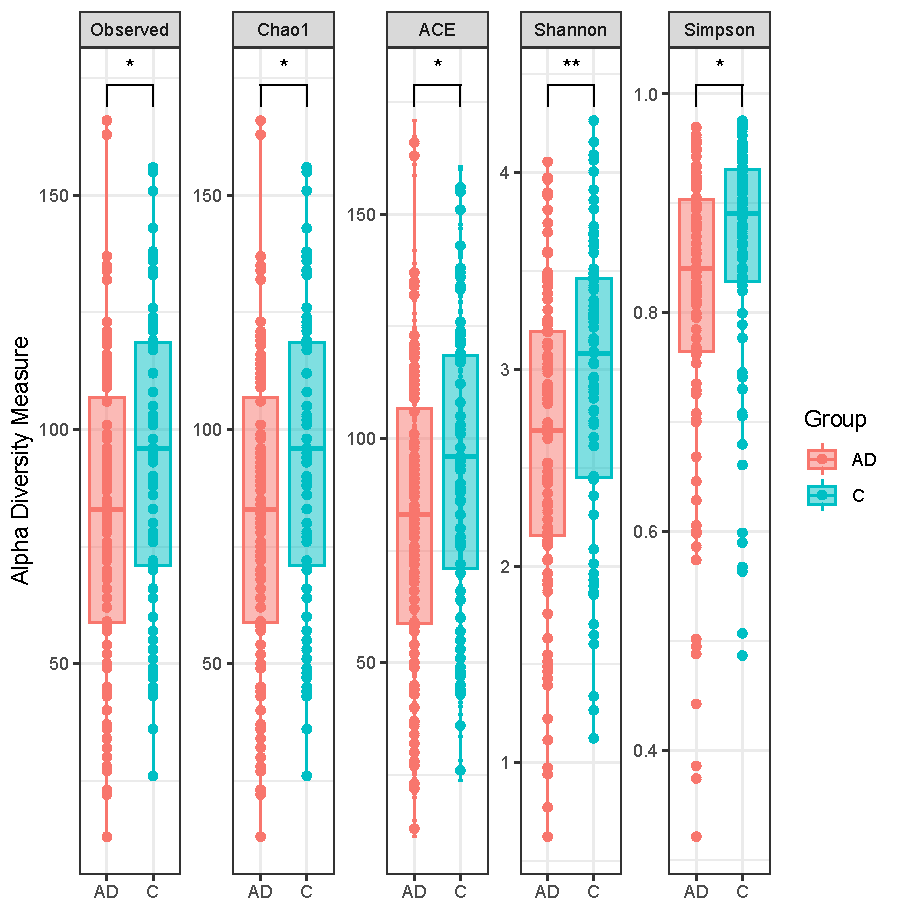
\includegraphics[scale=0.6]{plot/alpha.pdf}
	\caption{AD患者和对照组的Alpha多样性分析:两组间 Observed species、 ACE、 Chao1 以及 Shannon、Simpson 指数得分的箱式图:红色代表 AD 患者组,绿色代表健康对照组;箱子的上下限,分别是数据的上四分位数和下四分位数;箱子中间的一条线,是数据的中位数,代表了组内数据的平均水平;每个指数都使用 Wilcoxon 检验分析组间显著性差异,'**' 代表 p 值 < 0.01, '*' 代表 p 值 < 0.05 }
	\label{fig:alpha}
\end{figure}


对两组样本的数据进行 Beta 多样性分析,分别计算 Jaccard, Bray-Curtis, Unweighted UniFrac 和 Weighted UniFrac 距离,使用 PCoA 在二维平面投影(\autoref{fig:beta}),可知无论是否考虑物种丰度变化和物种进化关系,尽管组内个体存在差异,AD 患者组和健康对照组样本组成群落分布明显分开,组间微生物群落存在显著性差异(PERMANOVA 检验,p 值均小于 0.05)。

通过 Alpha 多样性和 Beta 多样性分析可以得知,AD患者会影响到人肠道菌群的整体结构,与健康对照组存在显著差异。


\begin{figure}[htb]
	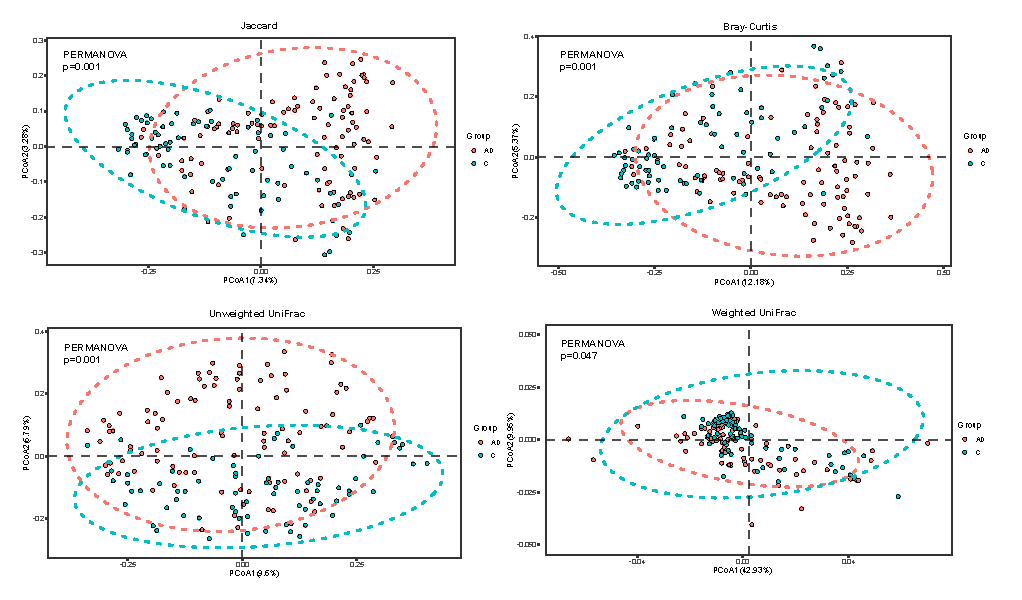
\includegraphics[width=\textwidth]{plot/beta.pdf}
	\caption{AD患者和对照组的Beta多样性分析:使用 PCoA 降维可视化不同距离算法下的样本距离:四张图依次从左到右,从上到下分别是:Jaccard, Bray-Curtis, Unweighted UniFrac 和 Weighted UniFrac 距离的 PCoA 降维距离分布图。横坐标(PCoA1)表示第一主成分,百分比则表示第一主成分对样品差异的贡献值;纵坐标(PCoA2)表示第二主成分,百分比表示第二主成分对样品差异的贡献值;每一个点代表一个样本,相同颜色的点来自同一个分组,红色代表 AD 患者组,绿色代表健康对照组;虚线椭圆代表的是 90\% 置信度下,对该组的总体区间估计;每张图的左上方标注了使用 PERMANOVA 检验得到的 p 值。 }
	\label{fig:beta}
\end{figure}

\subsection{阿尔茨海默症患者肠道微生物组成的相对失调}
对 ASVs 进行物种注释后,共得到 11 个门、17 个纲、43 个目、75 个科、208 个属以及 162 个种水平的菌种注释数据(\autoref{table:sum})。
\begin{generaltab}{两组样本得到的各注释水平的数目统计}{tab:heightweight}
	\begin{tabular}{c|c|c|c|c|c|c|c|c}
		\toprule
		Group & Kingdom & Phylum & Class & Order & Family & Genus & Species & ASVs\\
		\midrule
		D & 2 & 11 & 17 & 43 & 75 & 208 & 153 & 1456 \\ 
        C & 2 & 10 & 15 & 37 & 68 & 185 & 129 & 1254 \\ 
        SUM & 2 & 11 & 17 & 43 & 75 & 208 & 162 & 1584 \\     
		\bottomrule
		
	\end{tabular}
	\label{table:sum}
\end{generaltab}
使用LEfse进行组间物种组成差异分析,结果见\autoref{fig:diff},发现存在AD 患者组某些肠道微生物显著富集或减少。
在门水平上,发现 AD 患者肠道微生物中 Verrucomicrobiota(疣微菌门) 和 Actinobacteriota (放线菌门)比例显著增加;而 Firmicutes (厚壁菌门)显著下降。而 Firmicutes (厚壁菌门)显著减少。而 Proteobacteria (变形菌门)和 Bacteroidetes(拟杆菌门)没有显著变化,这与一些研究不一致\cite{zhuang22018gut}\cite{liu2019altered}。

\begin{figure}[htbp]
	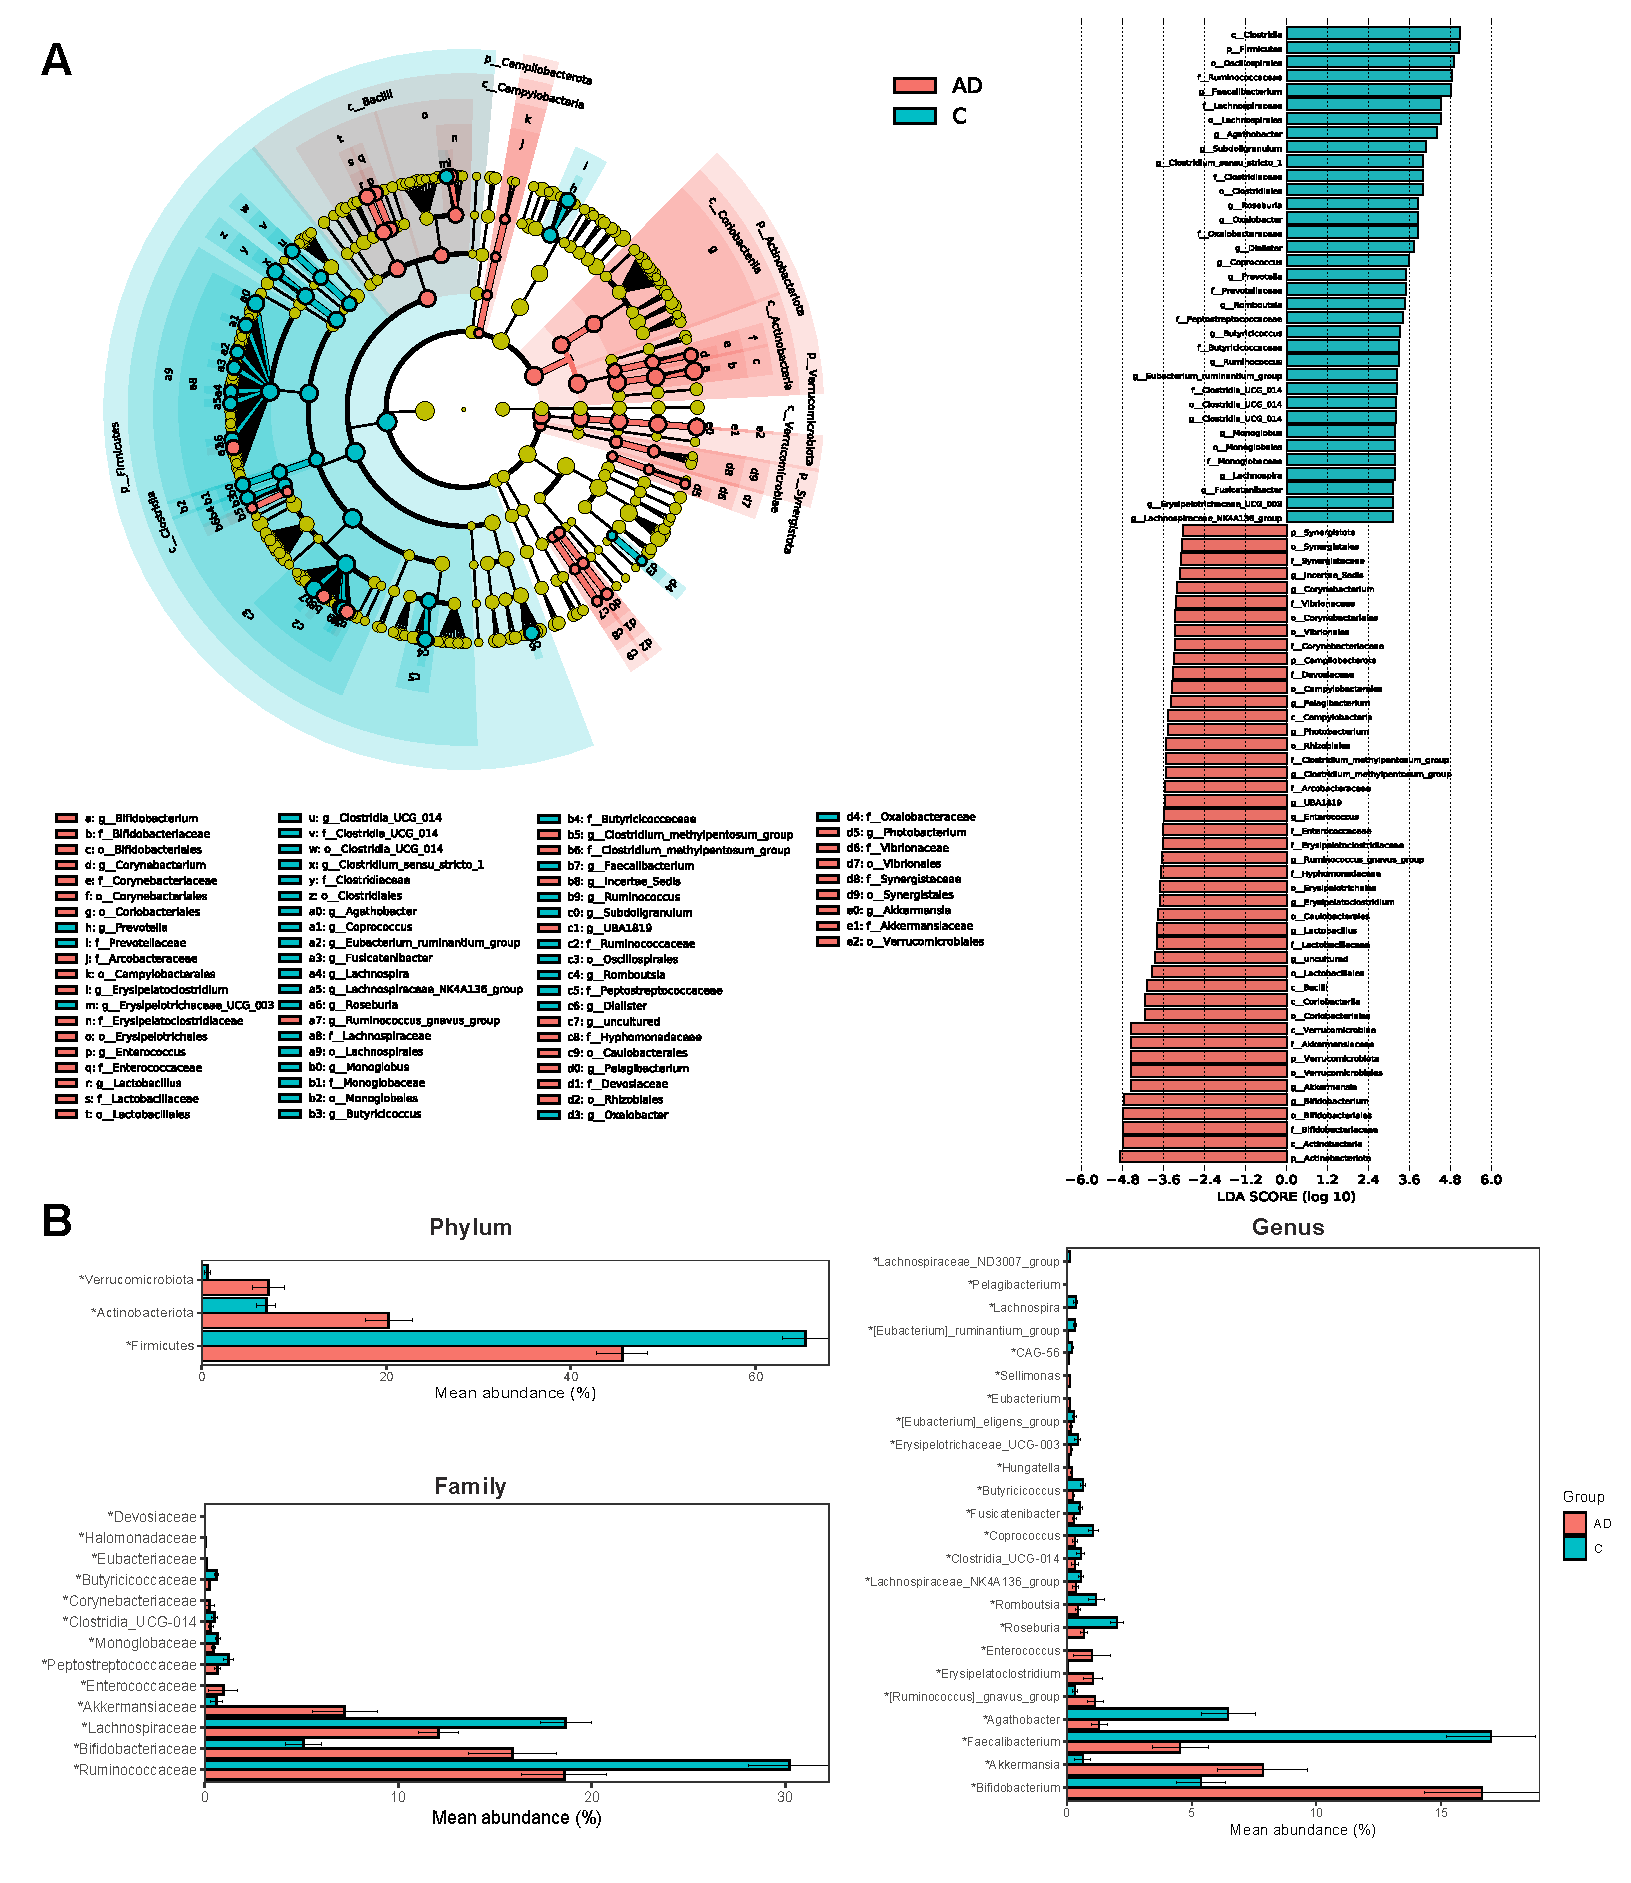
\includegraphics[width=\textwidth]{plot/difference analy.pdf}
	\caption{AD患者和健康对照组的组间物种组成差异分析:A) AD 患者与健康对照者肠道细菌物种的 LEfse 分析。 左图是 LEfse 绘制的进化分支图,由内至外辐射的圆圈代表了由门至属的分类级别,在不同分类级别上的每一个小圆圈代表该水平下的一个分类,小圆圈直径大小与相对丰度大小呈正比;着色原则:无显著差异的物种统一着色为黄色,差异物种 Biomarker 跟随组进行着色,红色节点表示在 AD 组别中起到重要作用的微生物类群,绿色节点表示在 C 组别中起到重要作用的微生物类群。图中英文字母表示的物种名称在右侧图例中进行展示。右图是 LDA 值分布柱状图,颜色代表对应分组,柱状图的长度代表差异物种的贡献度大小(即为 LDA Score),图中展示了 LDA Score 大于 3 的条件下不同组间丰度有显著差异的物种,即组内丰度显著高于其它组的 Biomarker。B)AD 患者与健康对照者肠道细菌的物种差异分析:使用 分别对门水平、科水平、属水平进行 Wilcoxon 检验,只展示 Bonferroni 矫正后的 p 值 <0.05 的物种。}
	\label{fig:diff}
\end{figure}


在科水平上,AD 患者肠道微生物中 Bifidobacteriaceae(双歧杆菌科)、Akkermansiaceae(艾克曼菌科)、Enterococcaceae(肠球菌科)、Corynebacteriaceae(棒状杆菌科)、Eubacteriaceae(优杆菌科) 在内的细菌家族比例显著增加;而 Ruminococcaceae(瘤胃菌科)、Lachnospiraceae(毛螺菌科)、Peptostreptococcaceae(消化链球菌科)、Monoglobaceae、Butyricicoccaceae 比例显著下降。Ruminococcaceae 和 Lachnospiraceae 生产不同类型的短链脂肪酸(SCFA)。在 SCFA 中,丁酸盐因其对维持健康的有益作用而在研究中受到特别关注。丁酸盐可影响胃肠生理学、肝脏代谢的外周免疫和血脑屏障的完整性,从而间接促进大脑功能,它可以驱动小胶质细胞的成熟,并且是维持成熟小胶质细胞所必需的\cite{fung2017interactions}。

在 Genus 水平上,Bifidobacterium(双歧杆菌属)、Akkermansia (艾克曼菌属)、[Ruminococcus]\_gnavus\_group(瘤胃球菌属)、Erysipelatoclostridium、Enterococcus(肠球菌属)、Hungatella 比例显著增加;Faecalibacterium(粪杆菌属)、Agathobacter、Roseburia(罗斯氏菌属)、Romboutsia、Lachnospiraceae\_NK4A136\_group(毛螺菌属)、Clostridia\_UCG-014、Coprococcus(粪球菌属)、Fusicatenibacter、Butyricicoccus、Lachnospira(毛螺菌属)、[Eubacterium]\_ruminantium\_group 比例显著下降。

在 AD 患者增加的属水平菌种中,Enterococcus 可在原代大鼠皮层神经元中产生早期阿尔茨海默样神经原纤维表位 \cite{vogt2017gut},在 AD 病因中可作为有害细菌。有趣的是 Bifidobacterium 和 Akkermansia 在传统上被认为是有益菌,却在 AD 患者中显著增加。Bifidobacteriaceae 和 Enterococcaceae 主要是产生乳酸,在 AD 患者中增加。Bifidobacteriaceae 主要是一种乳酸产生菌,对人类非常有益,并已被用作乳制品中的食品添加剂\cite{camfield2011dairy}。Kobayashi 等人\cite{kobayashi2017therapeutic}进行的一项初步临床研究发现,使用 Bifidobacterium breve A1 的口服补充剂可以通过抑制炎症和免疫反应基因的基因表达,改善认知功能,维持老年人的生活质量。Akkermansia 是一个专门降解粘蛋白的属,可利用粘蛋白衍生的糖,如岩藻糖,通过丙二醇途径生产丙酸盐\cite{ottman2017genome}。先前的研究表明,Akkermansia muciniphila(典型菌株)与预防肥胖、促进伤口愈合、增强抗肿瘤反应和诱导免疫反应有关\cite{everard2013cross} \cite{greer2016akkermansia}。令人惊讶的是,本文所用的数据表明 Bifidobacterium 和 Akkermansia 是 AD 患者肠道富集微生物群中最丰富的属之一。这表明两者可能在 AD 的发病和发展中起关键作用。

在减少的属水平菌种,Faecalibacterium (典型菌株 F.prausnitzii)是厚壁菌门的主要成员,被认为是健康肠道最重要的细菌指标之一,可调节肠道上皮水平的炎症\cite{sokol2008faecalibacterium},有研究也发现老年帕金森病患者 Faecalibacterium 比例下降,Bifidobacterium 增多\cite{scheperjans2015gut},先前的研究发现,Faecalibacterium 具有抗炎特性,因为其能够产生丁酸盐并诱导 耐受性细胞因子\cite{sokol2008faecalibacterium},这些变化都可能导致促炎性肠道环境,从而导致健康状况下降的老年人出现慢性低度炎症。Roseburia 属是属于产生 SCFA(尤其是丁酸)的共生细菌,可影响免疫维持、结肠运动和抗炎特性\cite{tamanai2017roseburia}。Coprococcus 粪球菌属是大肠中数量较少的细菌,从果糖中产生丁酸,从乳酸中产生丙酸(通过丙烯酸途径)\cite{reichardt2018specific}。Faecalibacterium 和 Coprococcus,与多个生活质量分数(quality-of-life ,QoL)呈正相关\cite{valles2019neuroactive}。Butyricicoccus 也是产生丁酸的菌属,发现丁酸菌与临床指标 MMSE、WAIS 和 Barthel 以及抗炎细胞因子 IFN-γ 呈正相关,与促炎细胞因子 TNF-α 呈负相关,Zhang 等人 \cite{zhang2017altered}的研究表明,与年龄匹配的对照组相比,AD 小鼠模型中的丁酸菌数量明显减少,与我们的数据相符。


或许正是因为丰度增加的菌群和丰度减少的菌群相互作用,导致 SCFA 的变化,可能参与了 AD 的发病和发展。



\subsection{基于肠道微生物标志物能有效鉴别阿尔茨海默症患者}
对 171 个样本的 ASV 丰度数据随机划分为训练集(n=85)和测试集(n=86),先使用全部属水平的丰度数据构建随机森林分类器,通过 MeanDecreaseAccuracy 指标排序,选取了最高的 15 个 属水平的丰度数据,重新构建随机森林分类器(命名为 MC),OOB 从 21.18\% 降到 17.65\%。热图(\autoref{fig:forest}C)展示了这些标志物在所有样本的分布情况。该随机森林分类器对于训练数据集的预测达到了 100\% 的精确度,对于测序数据集的预测则达到 0.78\% 的精确度,绘制 ROC 曲线(接收者操作特征曲线,receiver operating characteristic curve),其 AUC(Area Under Curve) 面积为 0.85(\autoref{fig:forest} B)。

利用 Wilcoxon 秩和检验挑选的组间有显著性差异的属水平特征,提取总丰度前 15 的特征,构建另一个随机森林分类器(命名为 WC),对于测序数据集的预测则达到 0.79\% 的精确度,绘制 ROC 曲线,其 AUC 面积为 0.88(\autoref{fig:forest} B)。WC 分类器的效果要好于 MC。

通过 WC 分类器的良好效果,可知利用肠道微生物标志物来区别 AD 患者和健康人是具有很大潜力的。
\begin{figure}[htb]
	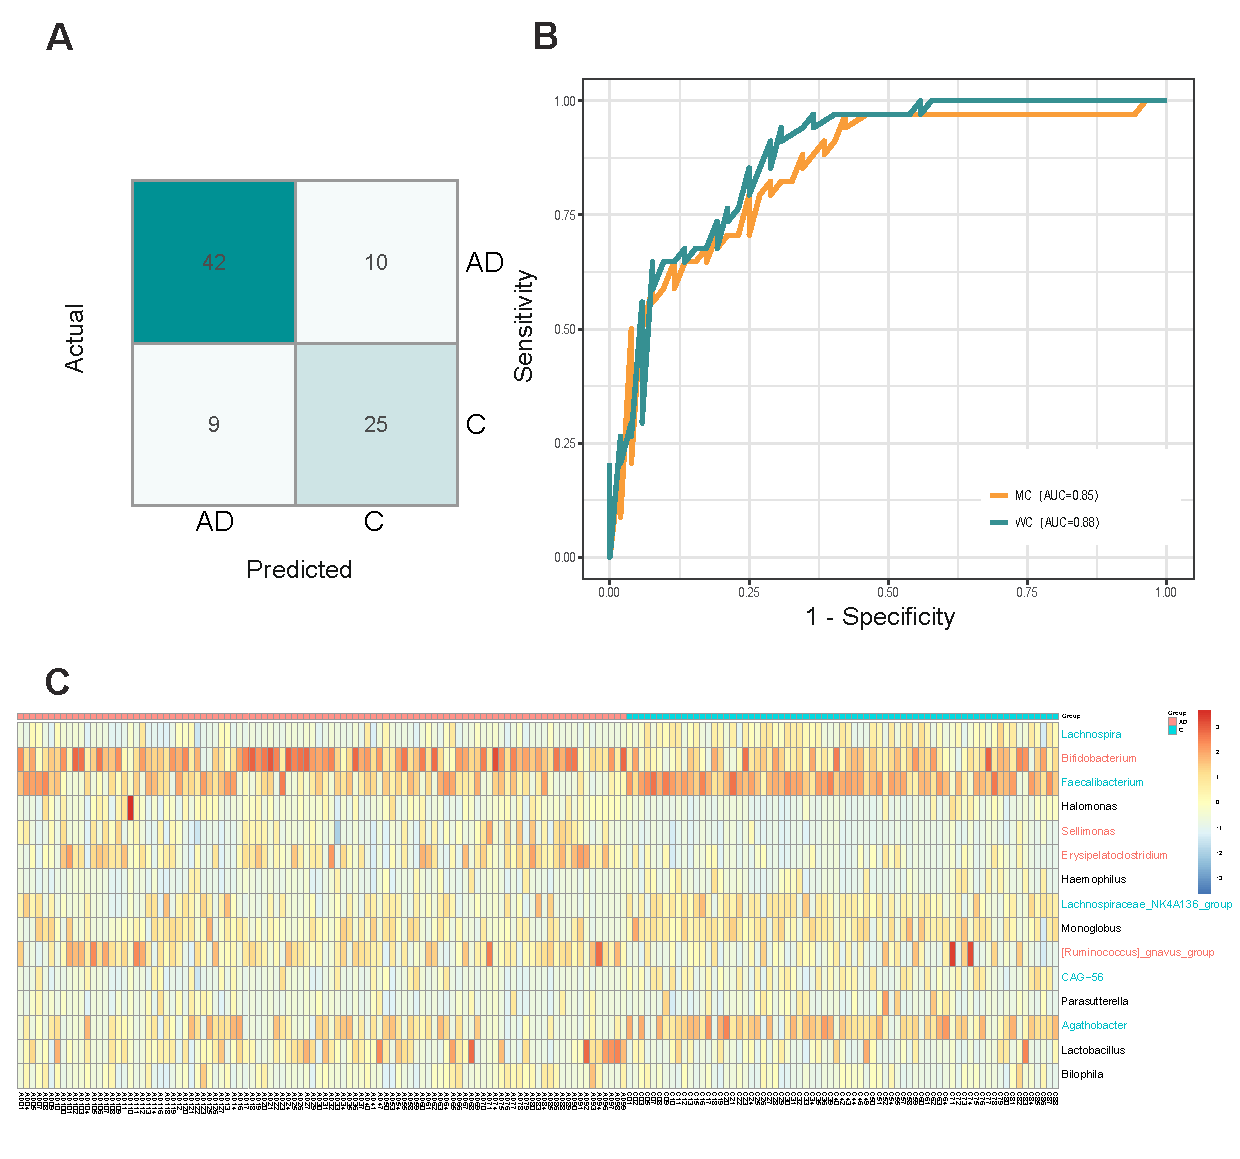
\includegraphics[width=\textwidth]{plot/RandomForest.pdf}
	\caption{随机森林分类器:A) WC 分类器针对测试集进行预测的混淆矩阵,横坐标代表预测的结果,纵坐标代表实际的标签,方块颜色代表对应区间的数目;B)MC分类器和WC分类器的ROC曲线图,黄色代表MC分类器,绿色代表WC分类器,图例旁标注有分类器各自的AUC值;C)MC分类器挑选的特征在所有样本的热力图,横坐标代表的是样本,红色代表AD组,绿色代表C对照组,纵坐标是通过 MeanDecreaseAccuracy 指标排序挑选的分值最高的 15 个 属水平}
	\label{fig:forest}
\end{figure}


\subsection{阿尔茨海默症患者的肠道微生物功能失调}
在二级 KEGG 通路上,比较了 45 个通路,并确定了 7 个在 AD 患者组和对照组之间具有明显差异丰度的 KEGG 类别,发现 AD 患者肠道菌群的 Glycan biosynthesis and metabolism(聚糖生物合成与代谢)、Carbohydrate metabolism(碳水化合物代谢),Chemical structure transformation maps (化学结构转换图)显著增加;而在 Cell motility(细胞运动)、“Folding,sorting and degration”(折叠分类讲解)、Energy metabolism(能量代谢),lipid metabolism(脂质代谢)显著减少(\autoref{fig:KEGG2})。

在三级 KEGG 通路上,比较了 163 个通路,并确定了 14 个在 AD 患者组和对照组之间具有明显差异丰度的 KEGG 类别,发现 AD 患者肠道菌群中的 Lipoic acid metabolism(硫辛酸代谢增加)、Other glycan degradation(其他聚糖降解)、Biosynthesis of terpenoids and steriods(萜类化合物和类固醇的生物合成)、Glycosaminoglycan degradation(糖胺聚糖降解)、Glycosphingolipid biosynthesis - globo and isoglobo series(糖鞘脂的生物合成 - globo 和 isoglobo 系列) 和 Glycosphingolipid biosynthesis - ganglio series (糖鞘脂的生物合成 - ganglio系列)共 6 条途经显著增加;而 Fatty acid biosynthesis(脂肪酸合成)、Peptidoglycan biosynthesis(肽聚糖生物合成)、Biotin metabolism (生物素代谢)、Porphyrin and chlorophyll metabolism(卟啉和叶绿素代谢)、Bacterial chemotaxis(细菌趋化性)、Flagellar assembly(鞭毛组件)、Sulfur relay system(硫磺中继系统)和 Thiamine metabolism(硫胺素代谢)共 8 条途径在 AD 患者肠道微生物群中显著减少(\autoref{fig:KEGG3})。

从而推知,肠道微生物群的功能失调可能参与 AD 的发病和发展。
\begin{figure}[htb]
	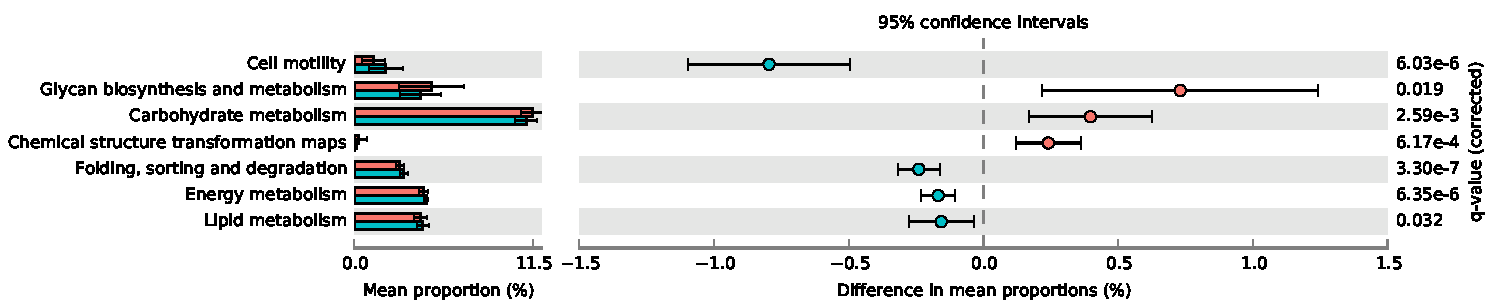
\includegraphics[width=\textwidth]{plot/KEGG2.pdf}
	\caption{AD患者和健康对照组在KEGG Level2 水平上的代谢通路差异}
	\label{fig:KEGG2}
\end{figure}
\begin{figure}[htb]
	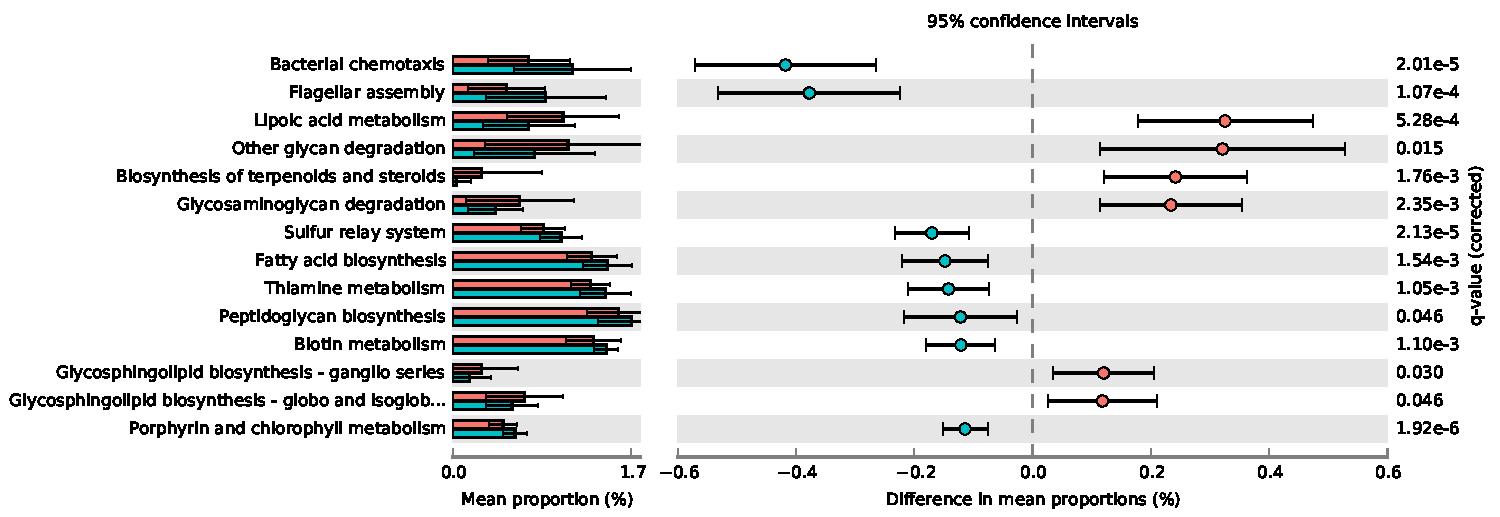
\includegraphics[width=\textwidth]{plot/KEGG3.pdf}
	\caption{AD患者和健康对照组在KEGG Level3 水平上的代谢通路差异}
	\label{fig:KEGG3}
\end{figure}


\section{总结与讨论}

近年来,多组学技术表明,肠道微生物群在促进人类健康方面起着至关重要的作用,因此它们常常被称为“被遗忘的器官”。越来越多的证据表明,肠道微生物群通过各种复杂机制构成维持肠道内环境稳定的关键因素\cite{wang2019sodium}\cite{la2018gut}\cite{mayer2015gut}。肠道微生物群不仅被认为是每种胃肠道疾病的促因,而且其影响的分析也被扩展到其他器官,如中枢神经系统(CNS)。大量研究已证实中枢神经系统(central nervous system,CNS)与胃肠道的双向活动,在肠道运动、吸收、内分泌、免疫功能,维持消化道内环境稳定等起重要作用。由于肠道微生物在脑-肠轴之间扮演着十分重要的角色, 我们可以将中枢神经系统、自主神经系统、肠神经系统、消化道以及种类繁多的肠道菌群视为一个整体,即菌-脑-肠轴 \cite{cryan2019microbiota} 。在这个系统中,信号转导发挥调节作用,这个作用是双向的。探索肠道微生物群在神经退行性疾病中的作用和机制是一个新兴的研究领域。肠-脑轴微生物群-肠-脑轴信号已经揭开了精神病学的一个新纪元,有望为精神疾病的诊断和治疗提供新的靶点,并破译其病因。

本文通过分析,发现 AD 患者的肠道微生物群在门、科和属的水平上的分布与健康对照组有着显著不同,物种丰富度降低,Alpha 多样性指数降低,Beta 多样性指数改变,与前人的研究相符合。Alpha 多样性和 Beta  多样性指数都提供了 AD 患者中肠道菌群组成和多样性改变的有力证据。观察到的 AD 患者肠道菌群整体结构失调也表明,与之相关的肠道微生物群的组成也发生了显著变化。通过组间物种组成差异分析,观察到在 AD 患者中 Faecalibacterium、Butyricicoccus、Coprococcus 等产丁酸的菌属减少,Bifidobacterium、Enterococcaceae 等乳酸产生菌显著增加,这貌似说明 AD 患者的肠道菌群倾向于产生乳酸分泌物。通过对肠道菌群的功能预测分析也表明,改变的肠道菌群与患者功能和代谢活动的改变有关,因为 SCFA 等代谢物的变化,可能参与了 AD 的发病和发展。


本文使用 AD 患者和健康对照组显著差异的 15 个菌属构建了随机森林分类器,显示了很好的预测性能。虽然没有对其他数据集进行进一步的测试,但也体现了使用肠道微生物作为生物标志物辅助 AD 患者早期非侵入性诊断的潜力。但要确定具体的微生物标志物,还需要更多的样本数据,针对具体地区进行探索,以保证模型的鲁棒性。


\section{代码公开}

本文涉及到的所有脚本和产生的数据文件都已上传至 Github 仓库,地址为\href{https://github.com/Achuan-2/Alzheimer_16S_analysis}{Achuan-2/Alzheimer\_16S\_analysis}



%生成参考文献
%使用方法:\bibliography{参考文件1文件名, 参考文献2文件名, ...}
\bibliography{Bibs/mybib}

% \begin{appendices}
% 	\section{这是第一个附录}
	
% 	这里是附录环境,其中的section、subsection、subsubsection已经变为附录的样式,并且会以这种样式加入目录中
% 	\subsection{附录可以有小节}
% 	\subsubsection{附录中也可以有小小节}\label{apxsubsubsec:appendix}
% 	\subsubsubsection{附录中也有小小小节}
% 	\verb|\autoref|无法识别Appendices环境,引用效果和正文一样,如\autoref{apxsubsubsec:appendix}。所以如果引用附录的话,建议直接使用附录~\ref{apxsubsubsec:appendix}~。
% \end{appendices}

\end{document}
